%% LyX 1.5.4 created this file.  For more info, see
%%           http://www.lyx.org/.
%% Do not edit unless you really know what you are doing.
%\documentclass[12pt,british,english,onecolumn]{IEEEtran}
\documentclass[british,english,journal]{IEEEtran}
\usepackage[T1]{fontenc}
\usepackage[latin9]{inputenc}
\usepackage{array}
\usepackage{amsmath}
\usepackage{graphicx}
\usepackage{setspace}
%\doublespacing
\usepackage{amssymb}
\newcommand{\tab}{\hspace*{2em}}

\makeatletter

%%%%%%%%%%%%%%%%%%%%%%%%%%%%%% LyX specific LaTeX commands.
%% Because html converters don't know tabularnewline
\providecommand{\tabularnewline}{\\}
%% A simple dot to overcome graphicx limitations
\newcommand{\lyxdot}{.}

%%%%%%%%%%%%%%%%%%%%%%%%%%%%%% User specified LaTeX commands.

% correct bad hyphenation here
%\hyphenation{op-tical net-works semi-conduc-tor}

\usepackage{geometry}

\geometry{verbose,letterpaper,tmargin=1cm,bmargin=2cm,
          lmargin=2cm,rmargin=2cm}

\makeatletter

%%%%%%%%%%%%%%%%%%%%%%%%%%%%%% LyX specific LaTeX commands.
%% Because html converters don't know tabularnewline
%% A simple dot to overcome graphicx limitations

%%%%%%%%%%%%%%%%%%%%%%%%%%%%%% User specified LaTeX commands.
\def\register{{\ooalign{\hfil\raise.07ex\hbox{\scriptsize R}\hfil
\crcr\mathhexbox20D}}}
\def\tm{\leavevmode\hbox{$\rm {}^{\scriptsize TM}$}}

\makeatother

\usepackage{babel}
\makeatother

\begin{document}

\title{{\Large The Synchronous Machine as a (Trivial kind of) Port Hamiltonian system.}}

\author{George Weiss\thanks{G.
Weiss is with the Department of Electrical Engineering Systems,
Faculty of Engineering, Tel Aviv University, Ramat Aviv 69978, Israel,
e-mail: gweiss@eng.tau.ac.il, Tel: 00972-3-640 5164.}}

%%%%%%%%%+%%%%%%%%%+%%%%%%%%%+%%%%%%%%%+%%%%%%%%%+%%%%%%%%%+%%%%%%%%%+
\maketitle

\section{Physical model of synchronous generator }
\subsection{The electrical part}
The mutual inductance between the field
coil and each of the three stator coils varies with the rotor
angle $\theta$:
\begin{eqnarray}
 & M_{af} & =M_{f}\mbox{cos}(\theta),\\
 & M_{bf} & =M_{f}\mbox{cos}(\theta-\frac{2\pi}{3}),\nonumber\\
 & M_{cf} & =M_{f}\mbox{cos}(\theta-\frac{4\pi}{3}) \nonumber
 \end{eqnarray}
 
 where $M_{f}>0$. The flux linkages of the windings are
\begin{eqnarray}
 & \Phi_{a} & =Li_{a}-Mi_{b}-Mi_{c}+M_{af}i_{f},\\
 & \Phi_{b} & =-Mi_{a}+Li_{b}-Mi_{c}+M_{bf}i_{f},\nonumber\\
 & \Phi_{c} & =-Mi_{a}-Mi_{b}+Li_{c}+M_{cf}i_{f}, \nonumber \\
 & \Phi_{f} & =M_{af}i_{a}+M_{bf}i_{b}+M_{cf}i_{c}+L_{f}i_{f} \nonumber
 \end{eqnarray}
where $i_{a}$, $i_{b}$ and $i_{c}$ are the stator phase currents
and $i_{f}$ is the rotor excitation current. Denote
\[ \Phi=\left[\begin{array}{c} \Phi_{a}\\ \Phi_{b}\\
   \Phi_{c}\end{array}\right],\quad i=\left[\begin{array}{c}
   i_{a}\\ i_{b}\\ i_{c}\end{array}\right]\]
and
\[ \widetilde{\mbox{cos}}\,\theta=\left[\begin{array}{c}
   \mbox{cos}\,\theta\\ \mbox{cos}(\theta-\frac{2\pi}{3})\\
   \mbox{cos}(\theta-\frac{4\pi}{3})\end{array}\right],\quad
   \widetilde{\mbox{sin}}\,\theta=\left[\begin{array}{c}
   \mbox{sin}\,\theta\\ \mbox{sin}(\theta-\frac{2\pi}{3})\\
   \mbox{\mbox{sin}}(\theta-\frac{4\pi}{3})\end{array}\right].\]

%%%%%%%%%+%%%%%%%%%+%%%%%%%%%+%%%%%%%%%+%%%%%%%%%+%%%%%%%%%+%%%%%%%%%+
% Figure 1
%
\begin{figure}
\begin{centering}
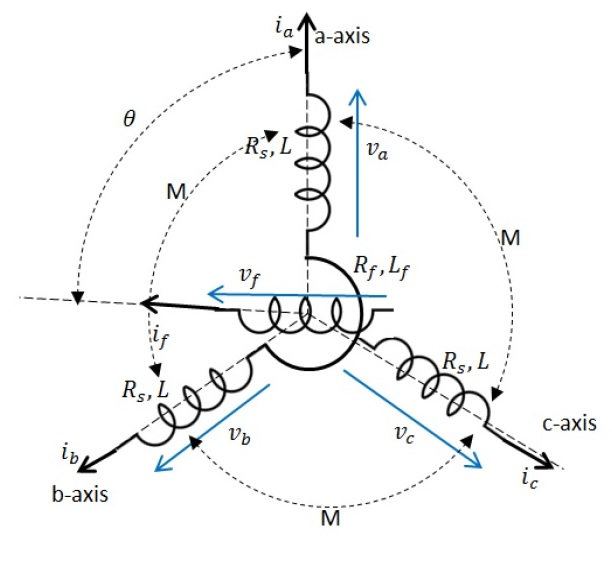
\includegraphics[scale=0.65]{FIG1} 
\par\end{centering}
\caption{\label{fig:Struct}Structure of an idealized three-phase
round-rotor synchronous generator.}
\end{figure}
%%%%%%%%%+%%%%%%%%%+%%%%%%%%%+%%%%%%%%%+%%%%%%%%%+%%%%%%%%%+%%%%%%%%%+

Assume that the neutral line is not connected, then
\[ i_{a}+i_{b}+i_{c}=0. \]
It follows that the stator flux linkages can be rewritten as
\begin{equation} \label{eq:Phi}
   \Phi = L_{s}i+M_{f}i_{f}\widetilde{\mbox{cos}}\,\theta,
\end{equation}
where $L_{s}=L+M$, and the field flux linkage can be rewritten as
\begin{equation}
   \Phi_{f} = L_{f}i_{f}+M_{f}\left\langle i,\,\widetilde{\mbox{cos}}
   \,\theta\right\rangle ,\label{eq:Phif} \nonumber
\end{equation}
where $\left\langle \cdot,\,\cdot\right\rangle$ denotes the
conventional inner product in $\mathbb{R}^{3}$. We remark that the
second term $M_{f}\left\langle i,\,\widetilde{\mbox{cos}}\theta\right
\rangle$ (called armature reaction) is constant if the three phase
currents are sinusoidal (as functions of $\theta$) and balanced. We
also mention that $\sqrt{\frac{2}{3}}\left\langle i,\,\widetilde{
\mbox{cos\,}}\theta\right\rangle$ is called the $d$-axis component of
the current.

Assume that the resistance of the stator windings is $R_{s}$, then
the phase terminal voltages $v=\left[\begin{array}{ccc} v_{a} & v_{b}
& v_{c}\end{array}\right]^{T}$ can be obtained from \eqref{eq:Phi} as
\begin{equation} \label{eq:stator}
   v = -R_{s}i-\frac{\mbox{d}\Phi}{\mbox{dt}} = -R_{s}i-L_{s}
   \frac{\mbox{d}i}{\mbox{dt}}+e,
\end{equation}
where $e=\left[\begin{array}{ccc}e_{a} & e_{b} & e_{c}\end{array}
\right]^{T}$ is the back emf due to the rotor movement given by
\begin{equation} \label{eq:ex}
   e = M_{f}i_{f}\dot{\theta}\widetilde{\mbox{sin}}\,\theta-M_{f}
   \frac{\mbox{d}i_{f}}{\mbox{dt}}\widetilde{\mbox{cos}}\,\theta.
\end{equation}
The voltage vector $e$ is also called no-load voltage, or synchronous
internal voltage.

We mention that, from \eqref{eq:Phif}, the field terminal voltage is
\begin{equation} \label{eq:rotor}
   v_{f} = -R_{f}i_{f}-\frac{\mbox{d}\Phi_{f}}{\mbox{dt}},
\end{equation}
where $R_{f}$ is the resistance of the rotor winding. 
%%%%%%%%%+%%%%%%%%%+%%%%%%%%%+%%%%%%%%%+%%%%%%%%%+%%%%%%%%%+%%%%%%%%%+
\subsection{The mechanical part}

The mechanical part of the machine is governed by
\begin{equation} 
   J\ddot{\theta} = T_{m}-T_{e}-D_{p}\dot{\theta},\label{eq:swing}
\end{equation}
where $J$ is the moment of inertia of all the parts rotating with
the rotor, $T_{m}$ is the mechanical torque, $T_{e}$ is the
electromagnetic toque and $D_{p}$ is a damping factor. $T_{e}$ can
be found from the energy $E$ stored in the machine magnetic field,
i.e.,
\begin{eqnarray*}
    & E & = \frac{1}{2}\left\langle i,\,\Phi\right\rangle +
      \frac{1}{2}i_{f}\Phi_{f}\\
    &   & = \frac{1}{2}\left\langle i,\, L_{s}i+M_{f}i_{f}
      \widetilde{\mbox{cos}}\,\theta\right\rangle\\
    &   & \qquad \quad + \frac{1}{2}i_{f}(L_{f}i_{f}+M_{f}\left
        \langle i,\,\widetilde{\mbox{cos}}\,\theta\right\rangle )\\
    &   & = \frac{1}{2}\left\langle i,\, L_{s}i\right\rangle +M_{f}
        i_{f}\left\langle i,\,\widetilde{\mbox{cos}}\,\theta \right
        \rangle +\frac{1}{2}L_{f}i_{f}^{2}.
\end{eqnarray*}
 From simple energy considerations we have
\[ T_{e} = \left.\frac{\partial E}{\partial\theta}\right|_{\Phi,\,
   \Phi_{f}\mbox{ constant}} \]
(because constant flux linkages mean no back emf, hence all the power
flow is mechanical). It is not difficult to verify (using the formula
for the derivative of the inverse of a matrix function) that this
is equivalent to
\[ T_{e}=-\left.\frac{\partial E}{\partial\theta}\right|_{i,\, i_{f}
   \mbox{ constant}}. \]
Thus,
\begin{equation} \label{eq:Te}
   T_{e} = -M_{f}i_{f}\left\langle i,\,\frac{\partial}{\partial
   \theta}\widetilde{\mbox{cos}}\,\theta\right\rangle =M_{f}i_{f}
   \left\langle i,\,\widetilde{\mbox{sin}}\,\theta\right\rangle .
\end{equation}


%%%%%%%%%+%%%%%%%%%+%%%%%%%%%+%%%%%%%%%+%%%%%%%%%+%%%%%%%%%+%%%%%%%%%+

\section{Deriving the dynamical equations}
In order to start deriving the dynamical equations, we will start with combing equations \eqref{eq:Phi}, \eqref{eq:stator} and \eqref{eq:rotor}:
\begin{eqnarray} \label{eq:ode}
 & e &= L_{s}\frac{\mbox{d}i}{\mbox{dt}}+R_{s}i+v, \\
 & -v_{f} &=\frac{\mbox{d}}{\mbox{dt}}\left( L_{f}i_{f}+M_{f}\left\langle i,\,\widetilde{\mbox{cos}}
   \,\theta\right\rangle \right) +R_fi_f\nonumber
 \end{eqnarray}
We will apply the Park transformation on it, where the Park transformation is:
\begin{equation} \nonumber
  U(\theta) = \sqrt{\frac{2}{3}}\begin{bmatrix}
 cos(\theta) & cos(\theta-\frac{2\pi}{3} & cos(\theta+\frac{2\pi}{3}\\ 
 -sin(\theta) & -sin(\theta-\frac{2\pi}{3} & -sin(\theta+\frac{2\pi}{3} \\ 
 \frac{1}{\sqrt{2}}&\frac{1}{\sqrt{2}}  & \frac{1}{\sqrt{2}}
\end{bmatrix}
\end{equation}

%%%%%%%%%+%%%%%%%%%+%%%%%%%%%+%%%%%%%%%+%%%%%%%%%+%%%%%%%%%+%%%%%%%%%+
% Figure 2
%
\begin{figure}
\begin{centering}
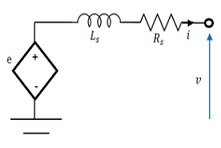
\includegraphics[scale=0.65]{FIG2} 
\par\end{centering}
\caption{\label{fig:StatorScheme}The stator scheme.}
\end{figure}
%%%%%%%%%+%%%%%%%%%+%%%%%%%%%+%%%%%%%%%+%%%%%%%%%+%%%%%%%%%+%%%%%%%%%+

After apply Part transformation on \eqref{eq:ode} we get:
\begin{equation} \label{eq:ParkOde}
L_sU(\theta)\frac{\mbox{d}i}{\mbox{dt}}+R_sU(\theta)i = U(\theta)e-U(\theta)v
\end{equation} 
\begin{equation}  \nonumber
\frac{\mbox{d}}{\mbox{d}\theta} \left[\begin{array}{c} i_{a}\\ i_{b}\\ i_{c} \end{array} \right]=U(\theta)\frac{\mbox{d}i}{\mbox{d}\theta}+\frac{\mbox{d}}{\mbox{d}\theta}U(\theta) i= U(\theta)\frac{\mbox{d}i}{\mbox{d}\theta}+\left[\begin{array}{c} i_{q}\\ -i_{d}\\ 0 \end{array} \right]
\end{equation} 
and because $\dot{f}(\theta(t))=\frac{\mbox{d}f(\theta(t))}{\mbox{d}\theta}\frac{\mbox{d}\theta}{\mbox{d}t}$ and that $\frac{\mbox{d}\theta}{\mbox{d}t} = \omega$, we have:
\begin{equation}  \nonumber
\frac{\mbox{d}}{\mbox{d}t} \left[\begin{array}{c} i_{d}\\ i_{q}\\ i_{0} \end{array} \right]=U(\theta)\frac{\mbox{d}i}{\mbox{d}t}+\omega \left[\begin{array}{c} -i_{q}\\ i_{d}\\ 0 \end{array} \right] 
\end{equation}
We can rewrite \ref{eq:ParkOde} as follows:
\begin{equation} 
L_s\frac{\mbox{d}}{\mbox{dt}}\begin{bmatrix} i_d \\ i_q \\ i_0 \end{bmatrix}-L_s\omega \begin{bmatrix} i_q \\ -i_d \\ 0 \end{bmatrix}+R_s \begin{bmatrix} i_d \\ i_q \\ i_0 \end{bmatrix} = \begin{bmatrix} e_d-v_d \\ e_q-v_q \\ i_0-v_0 \end{bmatrix}
\end{equation} 
Assuming that the neutral line is not connected, we obtain $i_0=0$, hence $e_0=v_0$. The dynamic equations for $i_d, i_q$ become
\begin{equation} \label{eq:idiqOde}
\frac{\mbox{d}}{\mbox{dt}}\begin{bmatrix} i_d \\ i_q \end{bmatrix}=\omega \begin{bmatrix} i_q \\ -i_d \end{bmatrix}- \frac{R_s}{L_s} \begin{bmatrix} i_d \\ i_q \end{bmatrix} +\frac{1}{L_s} \begin{bmatrix} e_d-v_d \\ e_q-v_q  \end{bmatrix}
\end{equation} 
Applying the Park transformation on \ref{eq:ex} becomes:
\begin{equation}   \label{eq:emf}
\begin{bmatrix} e_d \\ e_q \end{bmatrix}=-\sqrt{\frac{3}{2}}M
_f \begin{bmatrix} \dot{i_f} \\ \omega i_f \end{bmatrix}
\end{equation} 

for the dynamic equation of $i_f$, we go back to \ref{eq:ode} which becomes:
\begin{equation}  \nonumber
L_f \dot{i_f}+\sqrt{\frac{3}{2}}M_f i_d+R_fi_f=-v_f
\end{equation} 
whence 
\begin{equation}  \nonumber
\dot{i_f}=-\sqrt{\frac{3}{2}} \frac{M_f}{L_f} \left[ \omega i_q -\frac{R_s}{L_s}i_d+\frac{1}{L_s}(e_d-v_d) \right]-\frac{R_f}{L_f}i_f-\frac{1}{L_f}v_f
\end{equation}
Using here \ref{eq:emf}, we get:
\begin{equation}  \nonumber
\left( 1-\frac{3 M_f^2}{2 L_fL_s}\right)\dot{i_f}=-\sqrt{\frac{3}{2}} \frac{M_f}{L_f} \left[ \omega i_q -\frac{R_s}{L_s}i_d-\frac{1}{L_s}v_d \right]-\frac{R_f}{L_f}i_f-\frac{1}{L_f}v_f
\end{equation}
Denoting $\alpha = \left( 1-\frac{3 M_f^2}{2 L_fL_s}\right)^{-1}$
\begin{equation}  \label{eq:ifIde}
\dot{i_f}=-\alpha\sqrt{\frac{3}{2}}\frac{M_f}{L_f} \left[ \omega i_q -\frac{R_s}{L_s}i_d-\frac{1}{L_s}v_d \right]-\alpha\frac{R_f}{L_f}i_f-\alpha\frac{1}{L_f}v_f
\end{equation}
In order to get the  equation for $i_d,i_q$ and $i_f$, we will combine \ref{eq:idiqOde},\ref{eq:emf} and \ref{eq:ifIde} and we will get:
\begin{equation} \nonumber
\begin{split}
\frac{\mbox{d}}{\mbox{dt}}\begin{bmatrix} i_d \\ i_q \end{bmatrix}= & \omega \begin{bmatrix} i_q \\ -i_d \end{bmatrix}- \frac{R_s}{L_s} \begin{bmatrix} i_d \\ i_q \end{bmatrix} -\\
  \sqrt{\frac{3}{2}}\frac{M_f}{L_s} & \begin{bmatrix} -\alpha\sqrt{\frac{3}{2}}\frac{M_f}{L_f}\left(\omega i_q -\frac{R_s}{L_s}i_d -\frac{1}{L_s}v_d \right)-\alpha\frac{R_s}{L_f}i_f-\alpha\frac{1}{L_f}v_f \\ \omega i_f \end{bmatrix} \nonumber \\ -\frac{1}{L_s} \begin{bmatrix} v_d \\ v_q  \end{bmatrix} \nonumber
  \end{split}
\end{equation}

We can see that $\theta$ does not appear in these equations. This is one of the big achievements of the Park transformation.

If we put the dynamic equations in the matrix form we get:
\begin{equation} \label{eq:matrixOde}
\frac{\mbox{d}}{\mbox{dt}}\begin{bmatrix} i_d \\ i_q \\ i_f \end{bmatrix} = 
\mathcal{A}(\omega)\begin{bmatrix} i_d \\ i_q \\ i_f \end{bmatrix}+
\mathcal{B}(\omega)\begin{bmatrix} v_d \\ v_q \\ v_f \end{bmatrix} 
\end{equation}
Where 
\begin{equation} \nonumber
\mathcal{A} = 
\begin{bmatrix}
 -\alpha\frac{R_s}{L_s} & \alpha\omega & \alpha\sqrt{\frac{3}{2}}\frac{M_fR_f}{L_sL_f}  \\
 -\omega & -\frac{R_s}{L_s} & -\sqrt{\frac{3}{2}}\frac{M_s}{L_s}\omega \\
 \alpha\sqrt{\frac{3}{2}}\frac{M_fR_s}{L_fL_s} & -\alpha\sqrt{\frac{3}{2}}\frac{M_f}{L_f}\omega &-\alpha\frac{R_f}{L_f} 
 \end{bmatrix}
\end{equation}
and 
\begin{equation} \nonumber
\mathcal{B} = 
\begin{bmatrix}
 -\frac{\alpha}{L_s} & 0 & \alpha\sqrt{\frac{3}{2}}\frac{M_f}{L_sL_f}  \\
 0 & -\frac{1}{L_s} & 0 \\
 \alpha\sqrt{\frac{3}{2}}\frac{M_f}{L_fL_s} & 0 &-\frac{\alpha}{L_f} 
 \end{bmatrix}
\end{equation}
Donate $m=\sqrt{\frac{3}{2}}M_f$ 

After applying Park transformation on \ref{eq:Te} we get:
\begin{equation} \label{eq:Te}
   T_{e}  =M_{f}i_{f}
   \left\langle i,\,\widetilde{\mbox{sin}}\,\theta\right\rangle = -\sqrt{\frac{3}{2}}M_fi_fi_q=-mi_fi_q
\end{equation}
The kinetic energy of the machine is $E_{kin} =\frac{1}{2}J\omega ^2$. Then using equation \ref{eq:swing} 
\begin{equation}
\begin{split}
\dot{E_{kin}}  =  J\dot{\omega}\omega = J\omega\left(\frac{1}{J}\left(T_m-T_e-D_p\omega\right)\right) \\
 = \omega\left(T_M-T-e-D-p\omega\right)
 \\
= \omega\left(T_m+mi_fi_q-D_p\omega\right)
\end{split}
\end{equation}
Using this equation we can derive differential equation for $\theta$:
\begin{equation}
\dot{\omega}=\frac{1}{J}\left(T_m+mi_fi_q-D_p\omega\right)
\end{equation} 

now, we have the full differential equation that represents the machine behavior:
\begin{equation} \label{eq:fullOde}
\frac{\mbox{d}}{\mbox{dt}}\begin{bmatrix} i_d \\ i_q \\ i_f \\ \omega \end{bmatrix} = 
\tilde{\mathcal{A}}(\omega,i_f)\begin{bmatrix} i_d \\ i_q \\ i_f \\ \omega \end{bmatrix}+\tilde{\mathcal{B}}(\omega,i_f)\begin{bmatrix} v_d \\ v_q \\ v_f \\ T_m \end{bmatrix}
\end{equation}
where 
\begin{equation} \nonumber
\tilde{\mathcal{A}} = 
\begin{bmatrix}
 -\alpha\frac{R_s}{L_s} & \alpha\omega & \alpha m \frac{R_f}{L_sL_f} & 0 \\
 -\omega & -\frac{R_s}{L_s} & 0 &-m\frac{i_f}{L_s} \\
 \alpha m \frac{R_s}{L_sL_f} & -\alpha m \frac{\omega}{L_f} &-\alpha\frac{R_f}{L_f} & 0 \\
 0  & \frac{m}{J}i_f&0 &\frac{-D_p}{J} 
 \end{bmatrix}
\end{equation}
and 
\begin{equation} \nonumber
\tilde{\mathcal{B}} = 
\begin{bmatrix}
 -\frac{\alpha}{L_s} & 0 & \frac{\alpha m}{L_sL_f} & 0  \\
 0 & -\frac{1}{L_s} & 0 & 0 \\
 \alpha\frac{\alpha m}{L_fL_s} & 0 &-\frac{\alpha}{L_f} & 0\\
 0 & 0 &0 & \frac{1}{J}
 \end{bmatrix}
\end{equation}

\section{The System as port Hamiltonian Controlled  System}
The energy in the magnetic field is 
\begin{eqnarray*}
    & E & = \frac{1}{2}\left\langle i,\,L_si\right\rangle +M_{f}i_f\left\langle i,\,\widetilde{\mbox{cos}}(\theta)\right\rangle+\frac{1}{2}L_fi^2_f\\
    &   & = \frac{1}{2}\left\langle i,\,L_si\right\rangle mi_fi_d+\frac{1}{2}L_fi^2_f\\
    &   & = \frac{1}{2}L_s\left(i_d^2+i_q^2\right)mi_fi_d+\frac{1}{2}L_fi^2_f
\end{eqnarray*}
Donate $\mathcal{L} = \begin{bmatrix} L_s & 0 & m\\ 0 & L_s &0 \\ m & 0 & L_f \end{bmatrix}$, then:
\begin{equation} \label{eq:emag}
E_{mag}=\frac{1}{2}\left\langle \begin{bmatrix} i_d \\ i_q \\ i_f \end{bmatrix},\,\mathcal{L}\begin{bmatrix} i_d \\ i_q \\ i_f \end{bmatrix}\right\rangle 
\end{equation}

The rate of the magnetic energy changing is:
\begin{eqnarray*} \nonumber
& \dot{E_{mag}} & =\left\langle \frac{\mbox{d}}{\mbox{dt}}\begin{bmatrix} i_d \\ i_q \\ i_f \end{bmatrix},\,\mathcal{L}\begin{bmatrix} i_d \\ i_q \\ i_f \end{bmatrix}\right\rangle \\ \nonumber &   & =  \left\langle \mathcal{A}(\omega)\begin{bmatrix} i_d \\ i_q \\ i_f \end{bmatrix}+
\mathcal{B}(\omega)\begin{bmatrix} v_d \\ v_q \\ v_f \end{bmatrix} ,\,\mathcal{L}\begin{bmatrix} i_d \\ i_q \\ i_f \end{bmatrix}\right\rangle \\ 
\nonumber &   & =  \left\langle \mathcal{L}\mathcal{A}(\omega)\begin{bmatrix} i_d \\ i_q \\ i_f \end{bmatrix},\,\begin{bmatrix} i_d \\ i_q \\ i_f \end{bmatrix}\right\rangle+
\left\langle+
\mathcal{L}\mathcal{B}(\omega)\begin{bmatrix} v_d \\ v_q \\ v_f \end{bmatrix} ,\,\begin{bmatrix} i_d \\ i_q \\ i_f \end{bmatrix}\right\rangle
\end{eqnarray*}

Now, the total energy in the system is:
\begin{equation} \label{eq:totalEnergy}
E=\frac{1}{2}( 
\left\langle \mathcal{L}\begin{bmatrix} i_d \\ i_q \\ i_f \end{bmatrix},\,\begin{bmatrix} i_d \\ i_q \\ i_f \end{bmatrix}\right\rangle +J\omega^2
) = \left\langle \tilde{\mathcal{L}}X, X\right\rangle
\end{equation}
Where $\tilde{\mathcal{L}} = \begin{bmatrix} L_s & 0 & m & 0\\ 0 & L_s &0 & 0\\ m & 0 & L_f & 0\\ 0 &0 & 0& J\end{bmatrix}$ and $X = \begin{bmatrix} i_d \\i_q \\ i_f \\ \omega \end{bmatrix}$
We have:
\begin{equation} \label{eq:LA}
\tilde{\mathcal{L}}\tilde{\mathcal{A}} = \begin{bmatrix} -R_s & \omega L_s & 0 & 0\\
 -\omega L_s & -R_s & 0 &-m\omega \\
 0 & 0 & -R_f & 0\\
 0 & mi_f & 0 &-D_p \end{bmatrix}
\end{equation}
We can decompose as $\tilde{\mathcal{L}}\tilde{\mathcal{A}}(\omega,i_f)=\tilde{J}(\omega,i_f)+N$ where $\tilde{J}$ is skew-adjoint, and $N<0$.
Now, we can write our system as a port-Hamiltonian system: notice that $\left[\frac{\partial E}{\partial x}\right]^*=\tilde{\mathcal{L}}x$
\begin{equation}
\dot{x} = \tilde{\mathcal{A}}(\omega,i_f)x+\mathcal{B}(\omega)v=A\left[\frac{\partial E}{\partial x}\right]^*+\tilde{\mathcal{B}}v
\end{equation}
where $A=\tilde{\mathcal{L}}^{-1}\tilde{\mathcal{L}}\tilde{\mathcal{A}}\tilde{\mathcal{L}}^{-1} = \tilde{\mathcal{L}}^{-1}\tilde{J}(\omega,i_f)\tilde{\mathcal{L}}^{-1}+\tilde{\mathcal{L}}^{-1}N\tilde{\mathcal{L}}^{-1}$
Now, $\tilde{\mathcal{L}}^{-1} = \begin{bmatrix} \frac{\alpha}{L_s} & 0 & -\frac{\alpha m}{L_sL_f} & 0\\ 0 & \frac{1}{L_s} &0 & 0\\ -\frac{\alpha m}{L_sL_f} & 0 & \frac{\alpha}{L_f} & 0\\0 & 0 &0 & \frac{1}{J} \end{bmatrix}$:
To have a complete port-Hamiltonian system, we need the output:
\begin{equation}
y=\tilde{\mathcal{B}}^{*}\left[\frac{\partial E}{\partial x}\right]^*=\tilde{\mathcal{B}}^*\mathcal{L}x=\begin{bmatrix} -i_d \\-i_q \\ -i_f \\ \omega \end{bmatrix}
\end{equation}
Thus, we get the reasonable passivity inequality:
\begin{equation} \nonumber
\dot{E}\leq-v_di_d-v_qi_q-v_fi_f-T_m\omega
\end{equation}
To have a "normal" passive system, we would have to change the signs of $u_d,u_q$ and $
u_f$ in the input vector, hence to change the sign of $\tilde{\mathcal{B}}(\omega)$. Then $\tilde{\mathcal{B}}(\omega) = \tilde{\mathcal{L}}^{-1} $. 
After this change of sign, the system has the structure:
\begin{equation}
\begin{split}
\dot{x}=\tilde{\mathcal{A}}(\omega,i_f)x+\tilde{\mathcal{B}}v \\
y=x
\end{split}
\end{equation}
where $x=\begin{bmatrix} i_d \\i_q \\ i_f \\ \omega \end{bmatrix}$, $v=\begin{bmatrix} -v_d \\-v_q \\ -v_f \\ T_m \end{bmatrix}$.\\
To make the energy $E= \frac{1}{2}\left\langle \tilde{\mathcal{L}}X, X\right\rangle$ positive definite, we need $\tilde{\mathcal{L}}>0$, which equivalent to $m^2<L_fL_s$. \\
If $m=L_fL_s$ \, then we get a descriptor type system, we lose one state variable. \\ \\
Another way of writing the equations:
\begin{equation}
\begin{split}
\tilde{\mathcal{L}}\dot{x}=\tilde{\mathcal{L}}\tilde{\mathcal{A}}(\omega,i_f)x+v \\
y=x
\end{split}
\end{equation}

Clearly $\mathcal{L}\tilde{\mathcal{A}} = J(x)+N$, where $J+J^*=0$ and $N<0$ which implies that this system is globally asymptotically stable. 
\\
\\
To have a classical port Hamiltonian system, we would have to introduce $z = \tilde{\mathcal{L}}x$ and then $E= \frac{1}{2}\left\langle \tilde{\mathcal{L}}^{-1}z,z\right\rangle$, $\left[\frac{\partial E}{\partial z}\right]^*=\tilde{\mathcal{L}}^{-1}z$
\begin{equation}
\begin{split}
\dot{z}=(J+N)\tilde{\mathcal{L}}^{-1}z+v \\
y=\tilde{\mathcal{L}}^{-1}z
\end{split}
\end{equation}
\section{Synchronization with an infinite bus}
\end{document}